\begin{figure}[t]
\centering
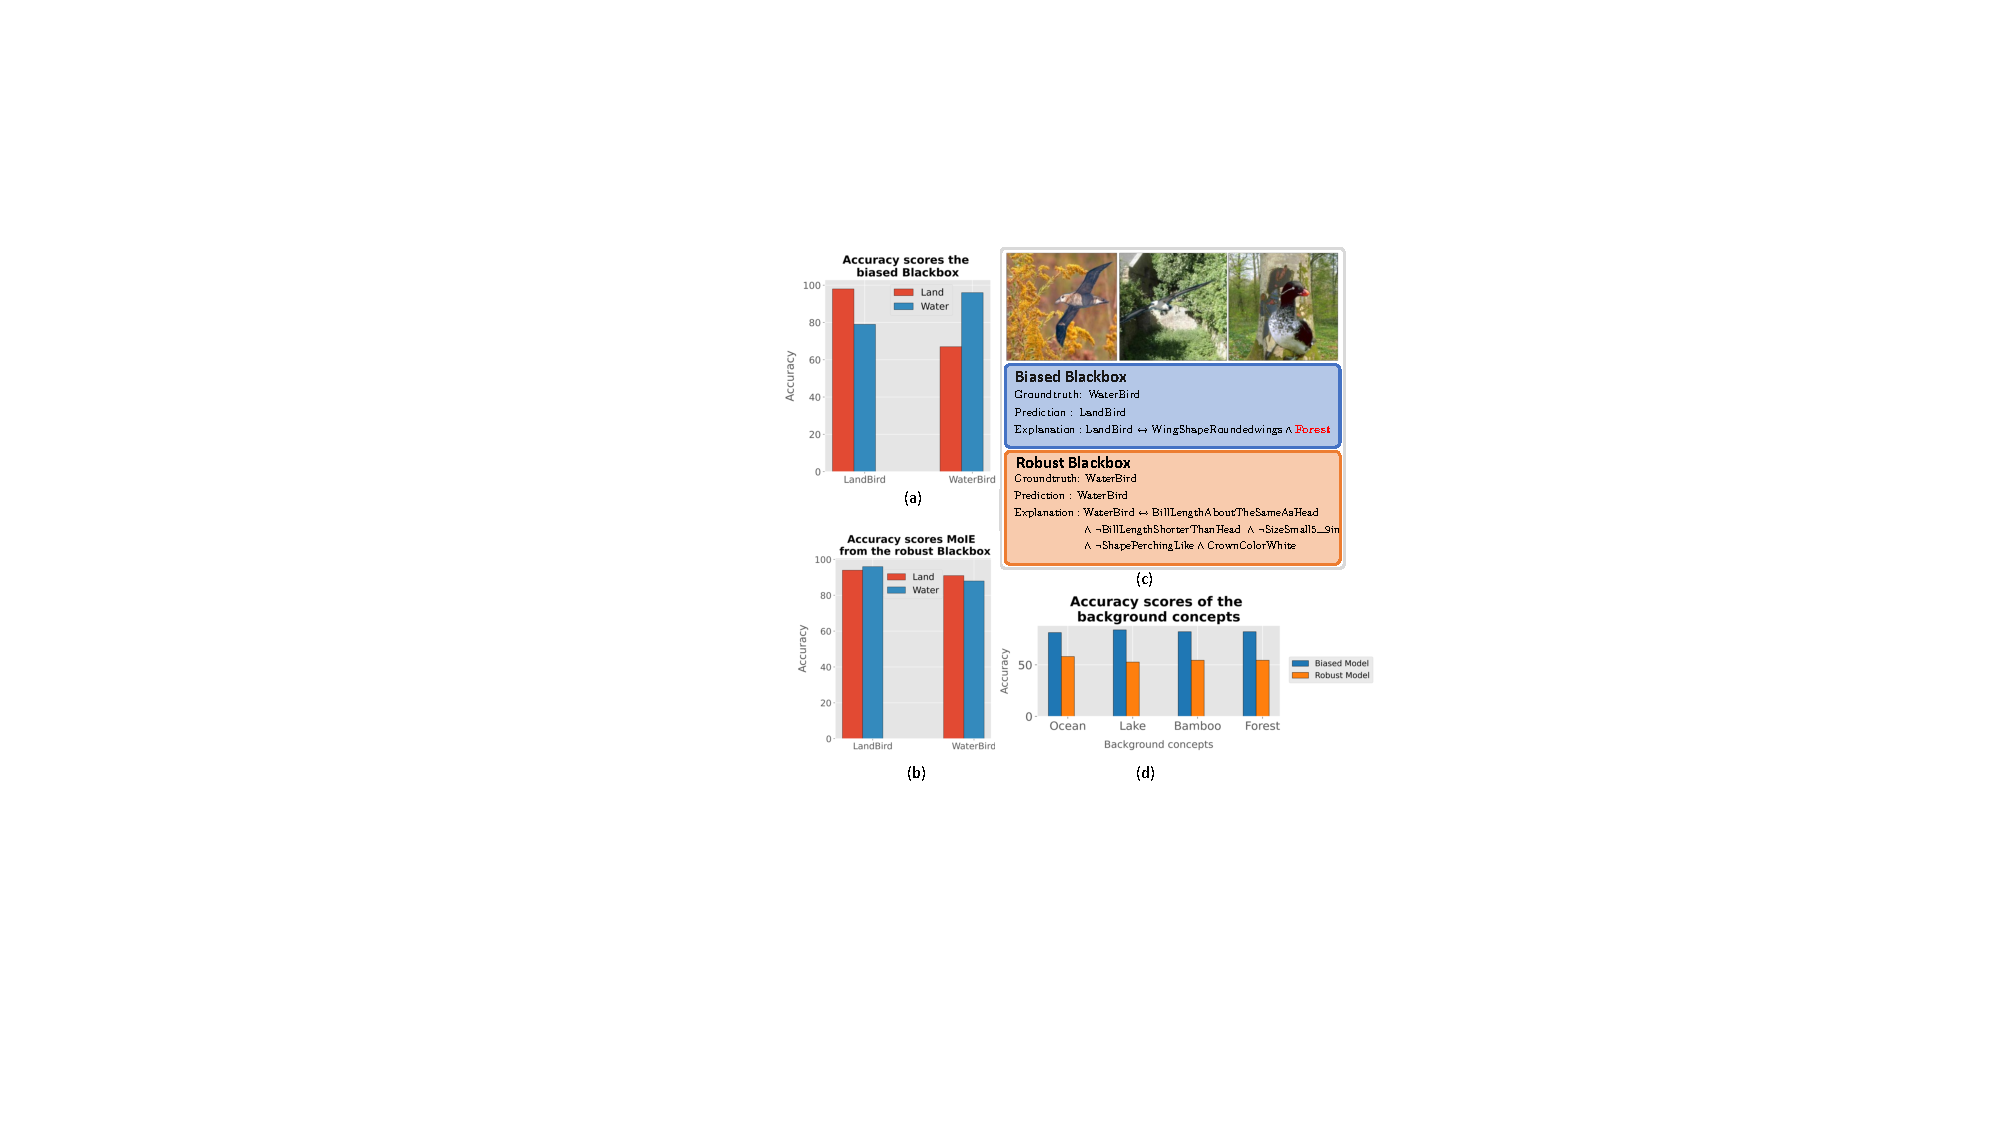
\includegraphics[width=1\textwidth]{figures/Final/shortcut.pdf}
\caption{Applying MoIE to eliminate shortcuts. (a) Performance of the biased Blackbox. 
(b) Performance of final MoIE, trained using the supervision of the robust Blackbox after removing the shortcuts using MDN. 
(c) Examples of samples and their explanations by the biased (top-row) and robust Blackboxes(bottom-row). 
(d) auroc and (e) accuracy metrics of the biased Blackbox (when the shortcuts are present) and the robust Blackbox (when the shortcuts are removed using MDN).
}
\label{fig:shortcut}
\end{figure}

To conduct this experiment, we create the Waterbirds dataset as in~\cite{sagawa2019dro} by spuriously correlating the images of birds from the Caltech-UCSD Birds-200-2011 dataset to the images of land and water background from the Places dataset. Specifically, we use forest and bamboo as the spurious land concepts for landbirds; ocean and lakes as the spurious water concepts for waterbirds. Thus, we have 112 visual concepts (108 concepts from CUB-200 and four new concepts for the background). We aim to identify each bird as a Waterbird or a Landbird. We use ResNet50 (\cite{he2016deep}) as the Blackbox $f^0$. The Blackbox quickly latches on the spurious background to classify the birds. As a result, the black box's accuracy varies for land-based subsets versus aquatic subsets of the bird species, as shown in figure \ref{fig:shortcut}a. The Waterbird on water is more accurate than on land ((96\%  vs. 67 \% in the orange bar in the figure \ref{fig:shortcut}a). We train $t$ to retrieve the concepts from the biased Blackbox. Next, we train our MoIE to explain the bird species using FOL. As per figure \ref{fig:shortcut}c (middle row), the FOL of a waterbird misclassified as a landbird captures the spurious concept \textit{forest}. Assuming the background concepts as metadata,  we aim to reduce the background bias from the representation of the Blackbox using metadata normalization (MDN) \cite{lu2021metadata}. Therefore, we leverage the MDN layers between two successive layers of the convolutional backbone to fine-tune the biased Blackbox. Next, we train $t$, using the embedding $\phi$ of the robust Blackbox. Figures \ref{fig:shortcut}d-e compare the auroc and accuracy scores of the spurious background concepts from the embedding $\phi$ of the biased and robust Blackboxes, respectively. The validation auroc (accuracy) of all the spurious concepts retrieved from the robust Blackbox fell well short of the predefined threshold 0.7 (70 \%) compared to the biased Blackbox. Finally, we re-train the MoIE distilling from the new robust Blackbox. Figure \ref{fig:shortcut}b illustrates that the accuracies of Waterbird on water vs. Waterbird on land become pretty similar (91\% -88 \%). The FOL from the robust Blackbox does not include any background concepts (Figure \ref{fig:shortcut}c, bottom row). Refer to the figure \ref{fig:spurious_flow} in Appendix \ref{app:shortcut} for the flow diagram of this experiment.